% Curves and Motion 500: the circle r = 2 sin(theta), centered at (0,1)
% with radius 1, with one point on it shown in polar coordinates.
\documentclass[border=4pt]{standalone}
\usepackage{tikz}
\begin{document}
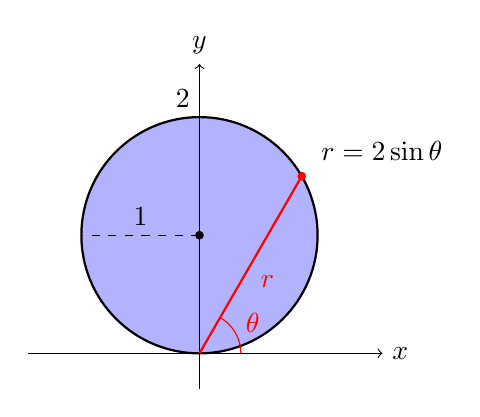
\begin{tikzpicture}[scale=1.5]
  \fill[blue!30] (0,1) circle (1);
  \draw[->] (-1.45,0) -- (1.55,0) node[right] {$x$};
  \draw[->] (0,-0.3) -- (0,2.45) node[above] {$y$};
  \draw[thick] (0,1) circle (1);
  % Radius of the circle.
  \filldraw (0,1) circle (.9pt);
  \draw[dashed] (0,1) -- (-1,1);
  \node[above] at (-0.5,1) {$1$};
  % A point on the circle at angle theta = 60 degrees: r = 2 sin(60) = sqrt(3).
  \draw[thick, red] (0,0) -- (60:1.732) node[midway, below right] {$r$};
  \filldraw[red] (60:1.732) circle (.9pt);
  \draw[red] (0.35,0) arc (0:60:0.35);
  \node[red] at (30:0.52) {$\theta$};
  \node[above left] at (0,2) {$2$};
  \node[above right] at (0.95,1.55) {$r=2\sin\theta$};
\end{tikzpicture}
\end{document}
